\newcommand{\plotfraction}{0.85}
Historically, dxex is based on PythonPDEVS~\cite{PythonPDEVS}.
Python is a good language for prototypes, but performance has proven insufficient to compete with other simulation kernels~\cite{MasterThesis}.
Dxex is a C++11-based implementation of PythonPDEVS, but implements only a subset of PythonPDEVS, while making some of its own additions.
So while the feature set is not too comparable, the architectural design, core simulation algorithm, and optimizations, are highly similar.

We will not make a detailed comparison with PythonPDEVS here, but only mention some supported features.
Dxex supports, similarly to PythonPDEVS, the following features: direct connection~\cite{SymbolicFlattening}, \textsf{Dynamic Structure DEVS}~\cite{DSDEVS}, termination conditions, and a modular tracing and scheduling framework~\cite{PythonPDEVS}.
But whereas PythonPDEVS only supports optimistic synchronization, dxex support multiple synchronization protocols (though only in parallel).
This is in line with the design principle of PythonPDEVS: allow users to pass performance hints to the simulation kernel.
In our case, a user can pass the simulation kernel the synchronization protocol to use for this model, or even switch the synchronization protocol during runtime.
Our implementation in C++11 also allows for optimizations which were plainly impossible in an interpreted language. Dxex will use new optimizations from the C++14 standard when possible.

Since there is no universal \textsf{DEVS} model standard, dxex models are incompatible with PythonPDEVS and vice versa.
This is due to dxex models being grafted on C++11, whereas PythonPDEVS models are grafted on Python.

In the remainder of this section, we will elaborate on our prominent new feature: support for multiple synchronization protocols within the same simulation tool, which are offered transparently to the model.

\subsection{Synchronization protocols}
We previously explained the existence of different synchronization protocols, each optimized for a specific kind of model.
As no single synchronization protocol is ideal for all models, a general purpose simulation tool should support multiple protocols.
Currently, most parallel simulation tools choose only a single synchronization protocol due to the inherent differences between protocols.
An uninformed choice on which one to implement is insufficient, as performance will likely be bad.
We argue that a real general purpose simulation tool should support sequential, conservative, and optimistic synchronization, as is the case for dxex.

These different protocols relate to three different model characteristics.
Conservative synchronization for when high lookahead exists between different nodes, and barely any blocking is necessary.
Optimistic synchronization for when lookahead is unpredictable, or there are rare (almost) instantaneous events.
Finally, sequential simulation is still required for models where parallelism is bad, where all protocols actually slow down simulation.

\subsubsection{Sequential}
Our sequential simulation algorithm is very similar to the one found in PythonPDEVS, including many optimizations.
Minor modifications were made, though, such that it can be overloaded by different synchronization protocol implementations.
This way, the \textsf{DEVS} simulation algorithm is implemented once, but parts can be overridden as needed.
In theory, more synchronization protocols (\textit{e.g.}, other algorithms for conservative synchronization) can be added without altering our design.

An overview of dxex's design is given in Figure~\ref{fig:class_diagram}.
It shows that there is a simulation \texttt{Core}, which simulates the \texttt{AtomicModel}s connected to it.
The superclass \texttt{Core} is merely the sequential simulation core, but can be used as-is.
Subclasses define specific variants, such as \texttt{ConservativeCore} (conservative synchronization), \texttt{OptimisticCore} (optimistic synchronization), and \texttt{DynamicCore} (\textsf{Dynamic Structure DEVS}).

\begin{figure}
    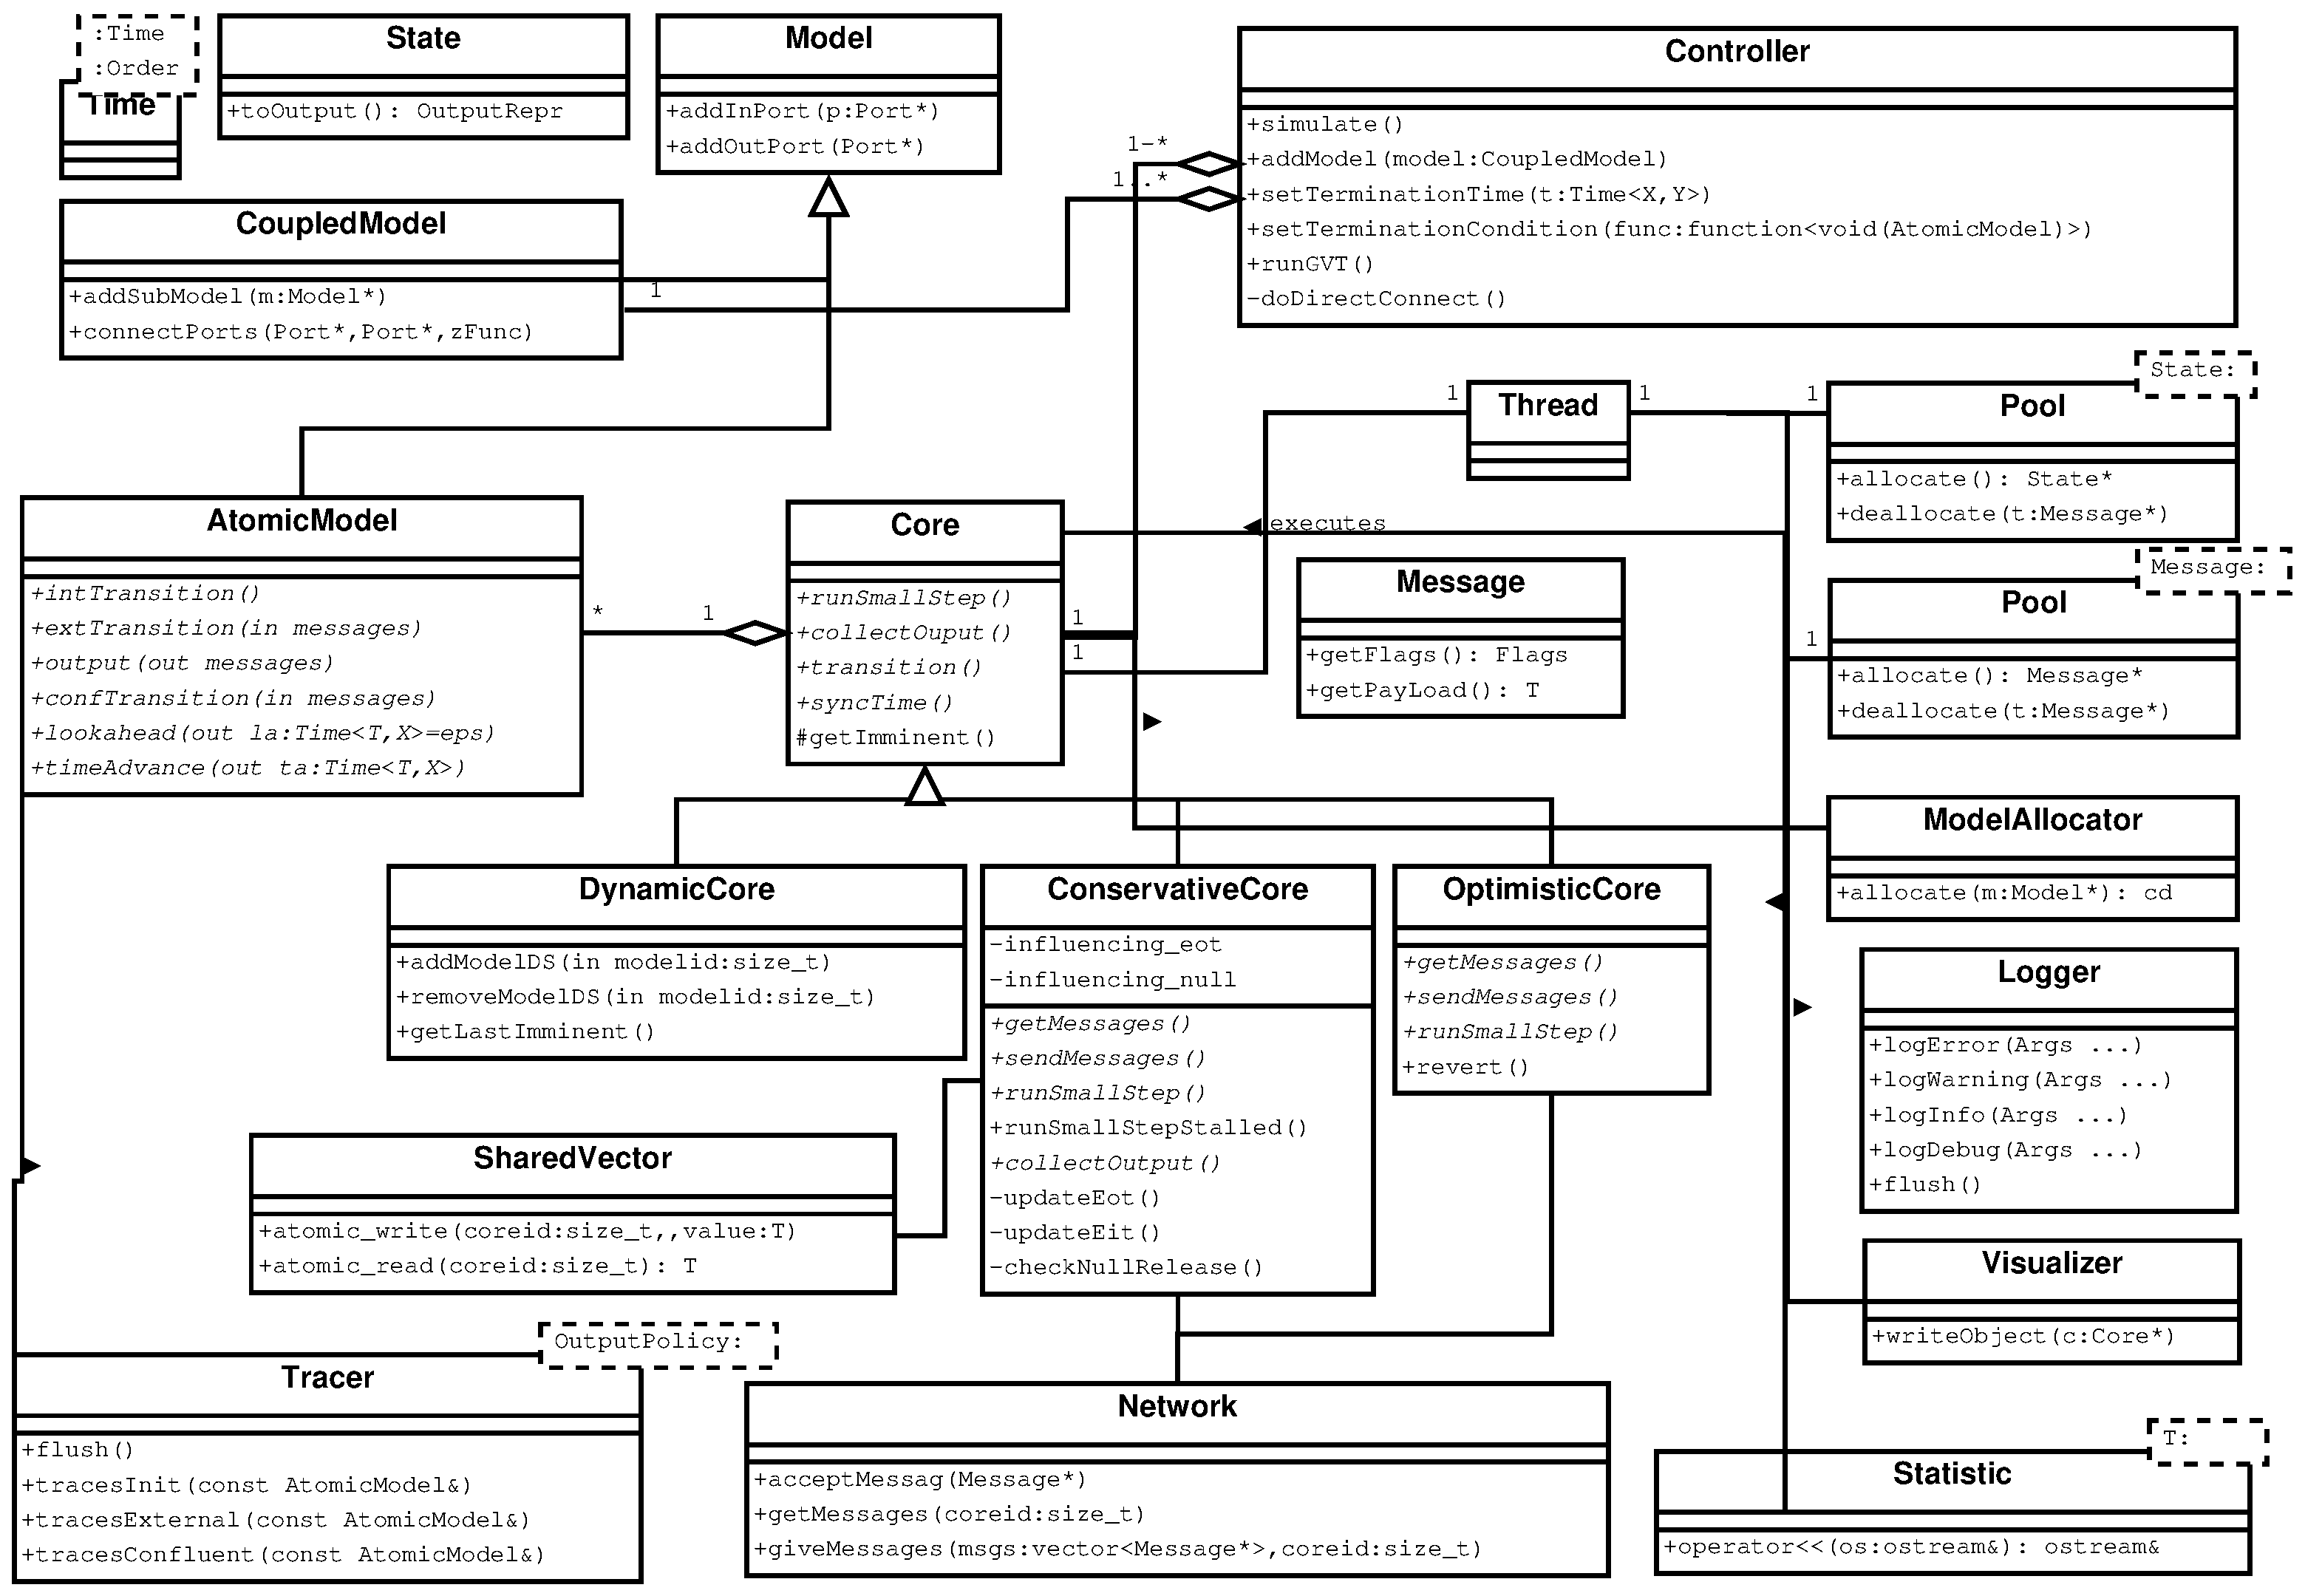
\includegraphics[width=\columnwidth]{fig/cores_class_diagram.eps}
	\caption{Dxex design.}
	\label{fig:class_diagram}
\end{figure}

\subsubsection{Conservative}
For conservative synchronization, each node must determine the nodes it is influenced by.
Each model needs to provide a lookahead function, which determines the lookahead depending on the current simulation state.
Within the returned time interval, the model promises not to raise an event.
A node aggregates this information to compute its earliest output time (EOT).
This value is written out in shared memory, where it can be read out by all other nodes.

Reading and writing to shared memory is done through the use of the new C++11 synchronization primitives.
Whereas this was also possible in previous versions of the C++ standard, by falling back to non-portable C functions, it was not a part of the C++ language standard.
C++11 further allows us to make the implementation portable, as well as more efficient: the compiler might know of optimizations specific to atomic variables or constant expressions which are heavily used in dxex.

\subsubsection{Optimistic}
For optimistic synchronization, each node must be able to roll back to a previous point in time.
This is often implemented through the use of state saving.
This needs to be done carefully in order to avoid unnecessary copies, and minimize the overhead.
We use the default: explicitly save each and every intermediate state.
Mattern's algorithm~\cite{mattern} is used to determine the GVT, as it runs asynchronously and uses only $2n$ synchronization messages.
Once the GVT is found, all nodes are informed of the new value, after which fossil collection is performed, and irreversible actions are committed.

The main problem we encountered in our implementation is the aggressive use of memory.
Frequent memory allocation and deallocation caused significant overheads, certainly when multiple threads do so concurrently.
This made us switch to the use of thread-local (using \texttt{tcmalloc}) memory pools.
Again, we made use of specific new features of C++11, that were not available in Python, or even previous versions of the C++ language standard.

\subsection{Transparency}
We define simulation kernel transparency as having a single model, which always can be executed on each supported synchronization kernel, without any modifications.
User should thus only provide one model, implemented in C++11, which can be either using sequential execution, using conservative synchronization, or using optimistic synchronization.
Switching between simulation kernels is as simple as altering the simulation termination time.
The exception is conservative synchronization, where a lookahead function is required, which is not used in other synchronization kernels.
Two options are possible: either a lookahead function must always be provided, even when it is not required and possibly not used, or we use a default lookahead function if none is defined.

Always defining a lookahead function might seem redundant, especially if users will never use conservative synchronization.
Especially since defining the lookahead is often non-trivial and dependent on intricate model details.
The more attractive option is for the simulation tool to provide a default lookahead function, such that simulation can run anyway, but likely not at peak performance.
Depending on the model, simulation performance might still be faster than sequential simulation. 

Defining a lookahead function is therefore recommended in combination with conservative synchronization, but is not a necessity, as a default $epsilon$ (\textit{i.e.}, the smallest representable timestep) is used otherwise.

\subsection{Features}
We will enumerate some of the extra features dxex offers to modellers.
\subsubsection{Runtime synchronization switching}
A user can request a runtime switch between synchronization protocols. A typical use case is when a significant slowdown is observed or memory usage reaches a certain treshold. The simulation engine will swap out the current kernels with new instances while preserving the state of the models and the simulation itself, and resume using the new synchronization protocol. There is no real limit on the number of switches, but the replacing and synchronizing of the kernels comes at a runtime cost that is dependent on the number of present kernels and the actual hardware the simulation runs on. A test case requires for 2 kernels an overhead approaching a second. This is an experimental but promising feature that can be used in an automated framework driven by machine learning techniques.
\subsubsection{Tracing}
Like PythonPDEVS dxex has full tracing capabilities supporting a wide number of output formats : Json, XML, Cell, console. The user can implement a new outputpolicy and use it in our modular tracing design. The tracing functionality itself is implemented asynchronous and thread-safe, the user does not need to use synchronization primitives. By overriding the output functions in the Message and State classes the user can generate model specific output for use with an existing tracing outputpolicy. Tracing can be completely disabled to maximize simulation performance should this be desired (e.g. benchmarks). 
\subsubsection{Memory Allocation}
As we will demonstrate in ~\nameref{sec:4-subsec:overhead-pgraph:memory} memory allocation is a performance bottleneck in simulation with high event frequency, especially in parallel with optimistic synchronization. Dxex has a modular allocation interface that separates the object creation in kernels and models from the actual implementation. This allows us by using a single compilation parameter to change the allocation strategy. This interface allows instrumentation of memory usage. Not only useful to detect memory leaks should this be a concern, it can also be of use to a model author to trace event creation in large models. The default implementation is the fastest common configuration verified by the benchmarks used in this publication.
\subsubsection{Model Allocation}
A model author can specify which kernel a model should be allocated to, should such manual intervention be required. This is handled by the default model allocator. If no preference is given a simple striping scheme is followed but this is not sufficient in most simulations to achieve a speedup in parallel. In Section \nameref{sec:4-performance} we analyse the performance impact of allocation schemes. By overriding the default allocator a model author can tune the allocation scheme for a specific model to maximize parallel speedup. This interface can be in future work also be used to employ graph algorithms for an automatic allocation scheme, for example one that avoids cycles in the resulting kernel dependency graph.
\subsubsection{Logging}
A high performance asynchronous buffered threaded logging module is used in dxex which offers a complete overview of the entire simulation. The logging functionality can be used in any model, it only requires linking to the dxex library. Logging statements are written to file with a granular level system. In case of a severe crash the logging system will ensure persistence of the log file itself up until the last statement. Logging can be completely disabled to remove the performance impact.
\subsubsection{Visualization and Statistics}
Tracing offers a black box view of a DEVS model in a simulation, with transitions, events and states recorded at each state change. Dxex supplements this optionally with more in depth insights into the actual simulation. 
The allocation of models across kernels is visualized at the end of a simulation along with the event trace of all events exchanged, including reverted events in optimistic. 
A user can then fine tune future allocation schemes. 

Invaluable during the development of dxex were runtime statistics collected by a simulation kernel. These record any measurable event in the simulation such as : events created/destroyed, inter kernel event frequency, reverts, GVT calculations, lookahead and eot values and insights into the fairness between the kernels themselves. Using this information it is possible to detect an imbalance between the simulation rounds that a single kernel executes compared to dependent or influencing kernels, observe how balanced inter kernel message traffic actually is during a simulation or measure the reverted simulation transition in optimistic synchronization.
The same information can, as in the visualization tool, be used programmatically to extend dxex with visualization software that shows the simulation from a white box perspective or allow activity tracking.
Figures \ref{fig:pholdtree_visualize_seq},\ref{fig:pholdtree_visualize_parDFS},\ref{fig:pholdtree_visualize_parBFS} give an example of the modular visualization output generated by dxex after simulation the PholdTree model. These figures demonstrate the effect of allocation visually, the high inter kernels event count will degrade performance, as we will demonstrate in 
\nameref{PholdTreeallocation} . Dotted lines represent connections between models that did not see events exchanged, directed edges represents events with frequency as weight and color to distinguish inter versus intra kernel events.
% Add figure
\begin{figure}
	\center
	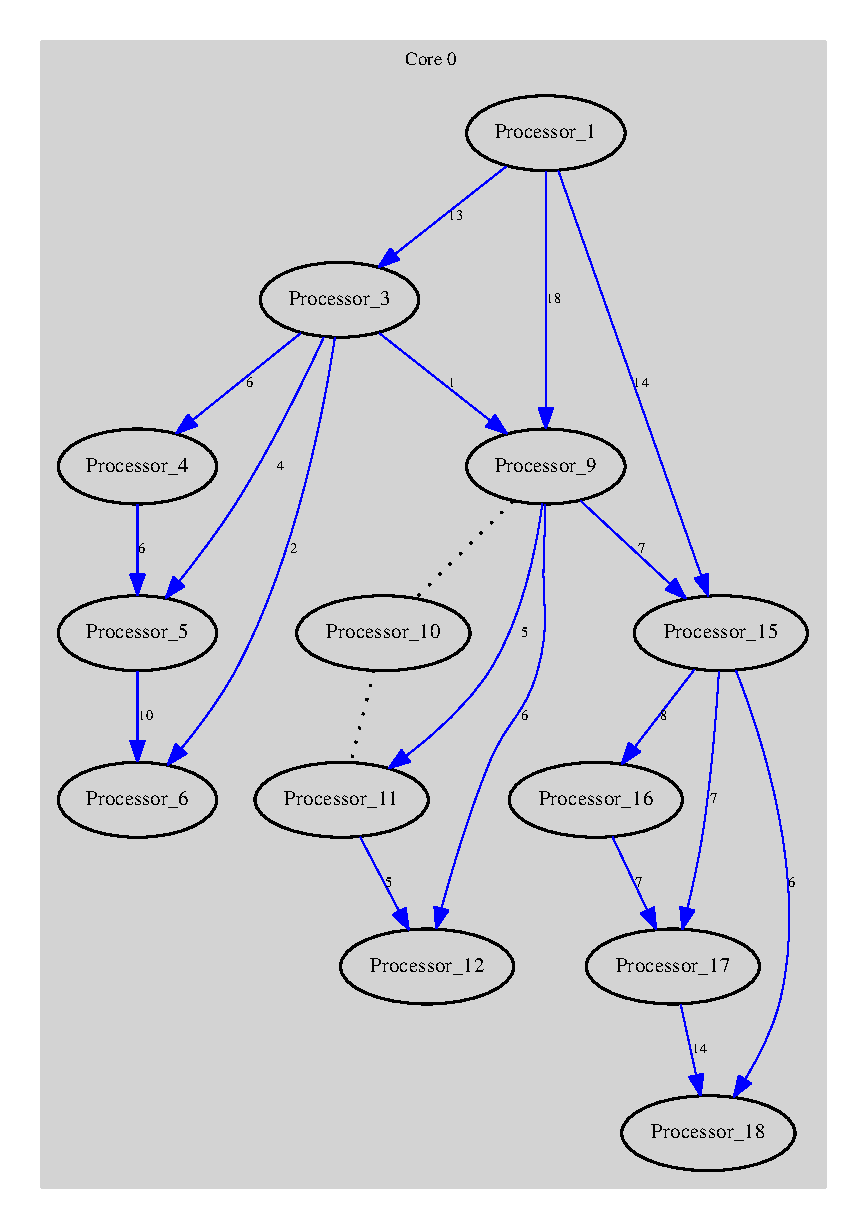
\includegraphics[width=\plotfraction\columnwidth, height=6cm, keepaspectratio]{fig/pholdtreed1n3t5000.eps}
	\caption{Visualization of PholdTree (d=1,n=3,t=5000) sequential simulation.}
	\label{fig:pholdtree_visualize_seq}
\end{figure}
\begin{figure}
	\center
	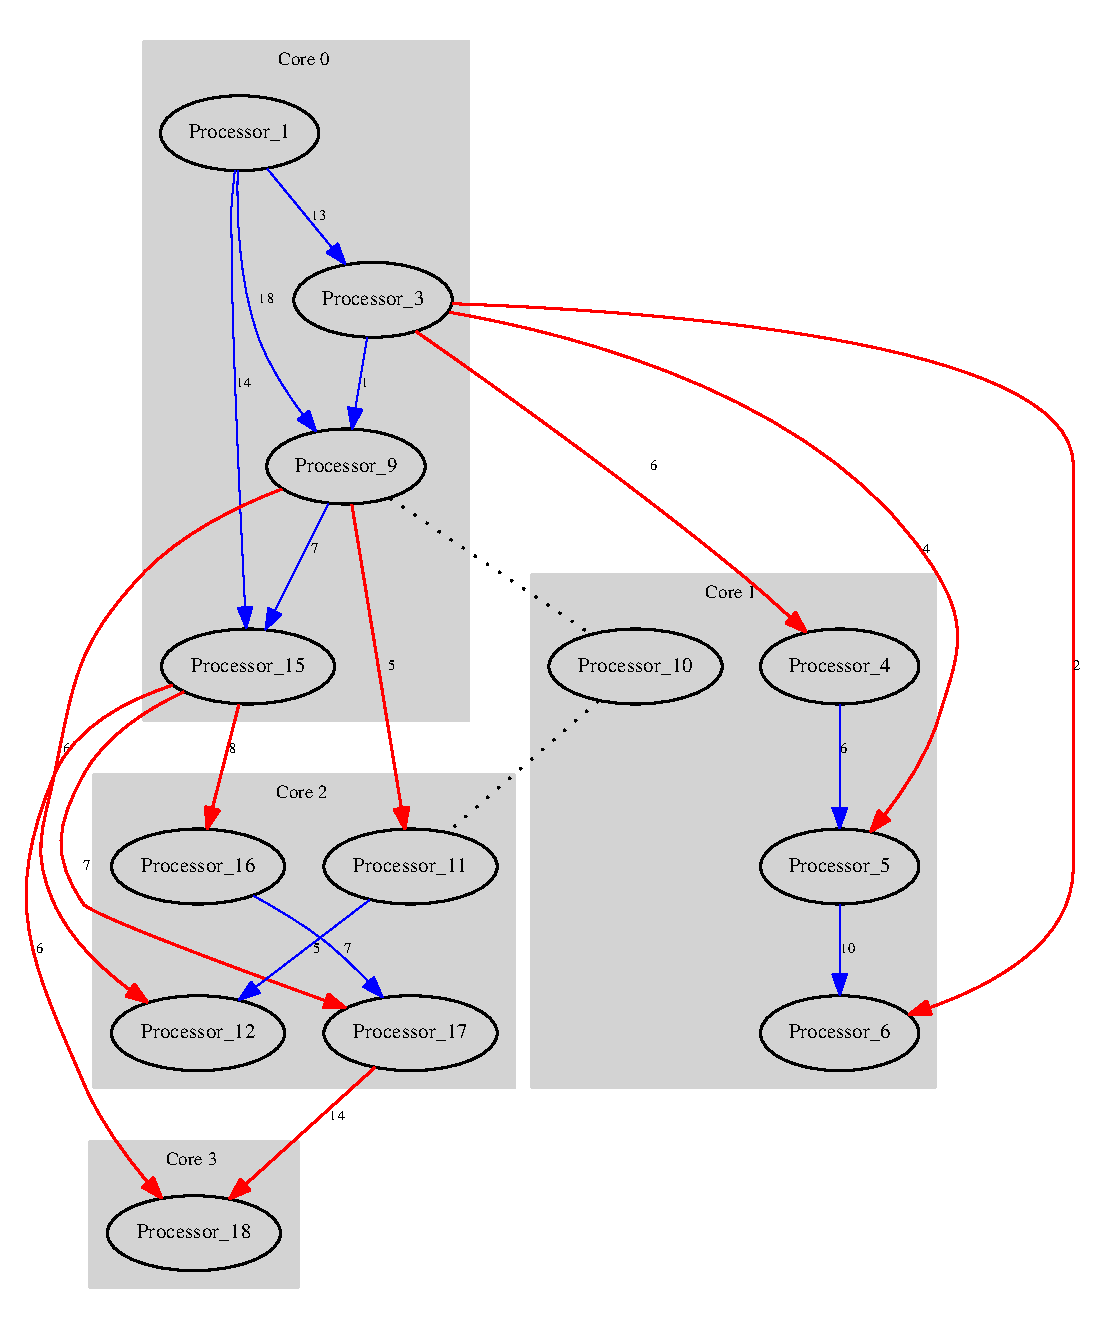
\includegraphics[width=\plotfraction\columnwidth,  height=6cm, keepaspectratio]{fig/pholdtreed1n3t5000c4BFS.eps}
	\caption{Visualization of PholdTree (d=1,n=3,t=5000) parallel simulation with breadth first allocation and 4 kernels.}
	\label{fig:pholdtree_visualize_parBFS}
\end{figure}
\begin{figure}
	\center
	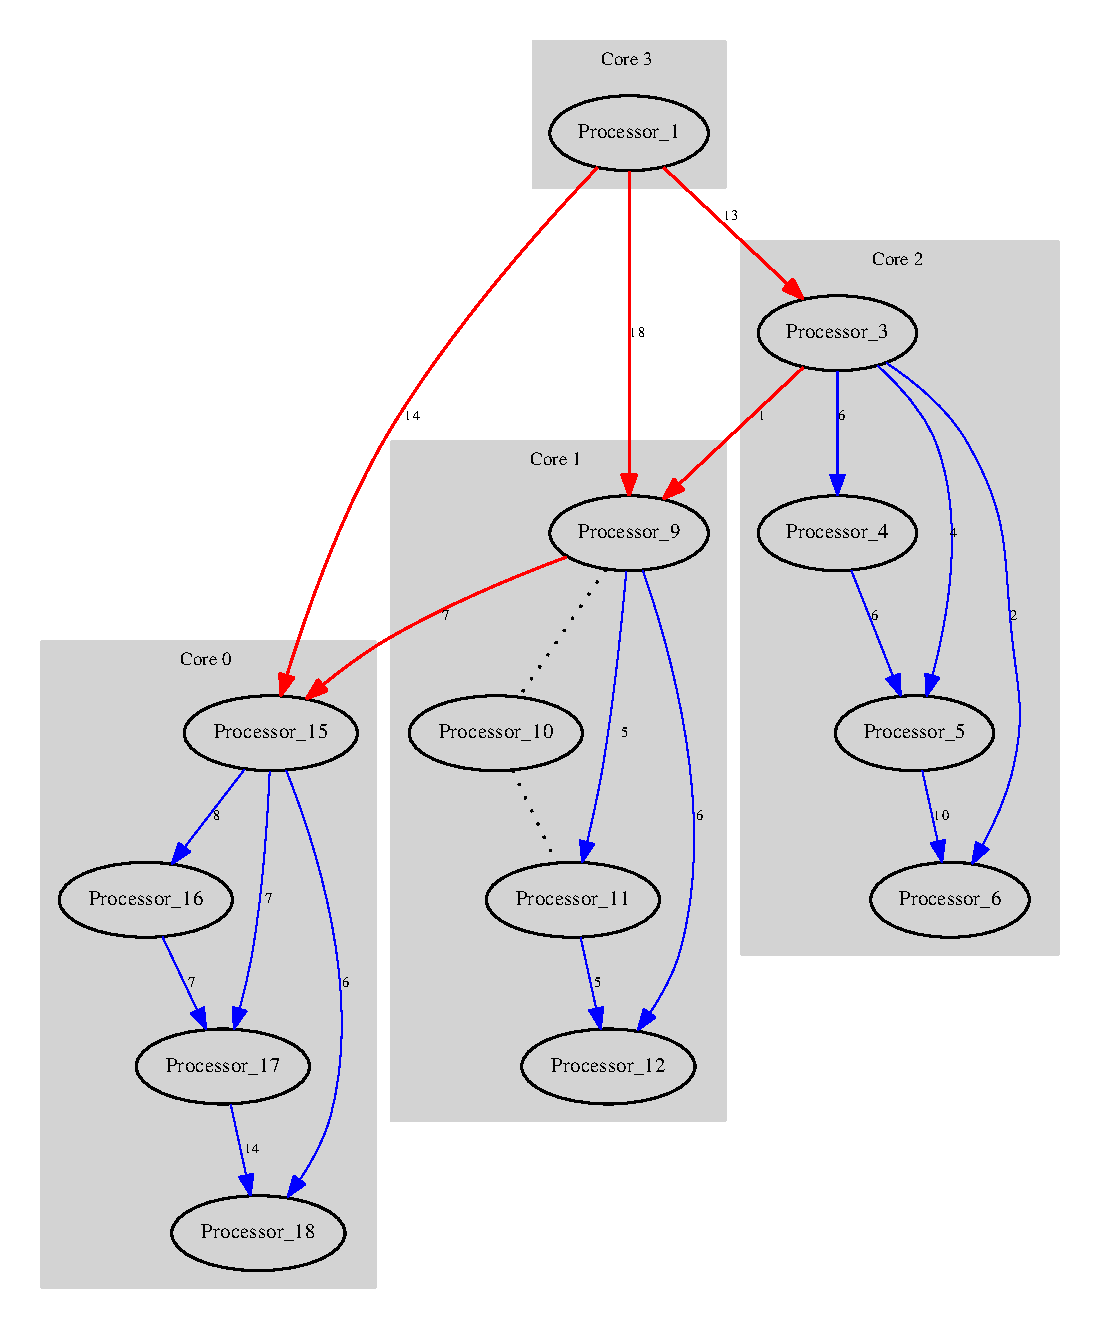
\includegraphics[width=\plotfraction\columnwidth,  height=6cm, keepaspectratio]{fig/pholdtreed1n3t5000c4DFS.eps}
	\caption{Visualization of PholdTree (d=1,n=3,t=5000) parallel simulation with depth first allocation and 4 kernels.}
	\label{fig:pholdtree_visualize_parDFS}
\end{figure}